% Chapter Template
\chapter{State of the art techniques}

\label{Chapter3} % Change X to a consecutive number; for referencing this chapter elsewhere, use \ref{ChapterX}

\lhead{Chapter 3. \emph{State of the art techniques}} % Change X to a consecutive number; this is for the header on each page - perhaps a shortened title

\section{Human Motion Understanding} % Main chapter title
 Human motions are rich in information. It conveys to the receiver the emotion, the attitude, the deeds and even the health of the human. Without understanding completely the human motion, it is not possible to achieve a very good HRI system.  Vision based motion capture and analysis has been studied widely and a condensed summary of all the approaches developed during the past two decades until 2000 have been presented by Moeslund et al. in \cite{Moeslund2001231} followed by the study of advancements during the years 2000-2006 in the survey \cite{Moeslund200690}. In the former the authors reviewed more than 130 publications while in the latter a review of over 300 publications was presented. This shows the rapid advancements in the study of the human motion in the recent times. Another work by Ronald Poppe \cite{Poppe20074} on the overview of vision based human motion analysis approached the problem into two discrete problems of modeling and estimation while also discussing the model free approaches to motion analysis. In this section an overview of the various approaches for pose estimation from RGB-D data and the gesture recognition are covered.
\subsection{Human Pose Estimation}
\label{sec:humanpose}
The surveys \cite{Moeslund2001231}\cite{Moeslund200690}\cite{Poppe20074} cited previously have investigated vision based human motion capture and analysis in general, however our particular focus is to use RGB-D sensors (presented in Section~\ref{ssec:rgbd_sensors}) to this purpose. Human pose estimation has traditionally suffered from two main problems
\begin{itemize}
\item Necessary to adopt an initialization pose.
\item Losing track after a few frames.
\end{itemize}
So alternative techniques which do not require to adopt an initialization pose and estimate pose from single depth images first appeared in the works of Shotton et al., \cite{shotton2013real}.
\subsubsection{Estimation from Single Depth Images}
 The initial publication by the Xbox team \cite{Kinect2014} appeared in \cite{shotton2013real} where real time human pose estimation in parts using single depth images has been proposed. An extension of this work has been published recently by the Microsoft computer vision research group \cite{shotton2013efficient}. This study proposes two approaches for human pose estimation which are capable of accurately predicting the 3D positions of body joints using single depth images without using any temporal information. The two methods also share their use of a very large, realistic, synthetic training corpus, generated by rendering depth images of humans. Each render is assigned randomly sampled parameters including body shape, size, pose, scene position, etc., thus generating quickly and cheaply hundreds of thousands of varied images with associated ground-truth (the body part label images and the set of 3D body joint positions). This enables to train deep random forests \cite{breiman2001random}, without the risk of overfitting, that can naturally handle a full range of human body shapes undergoing general body motions, self-occlusions, and poses cropped by the image frame. By using simple depth pixel comparison features, and parallelizable decision forests, both approaches could run in realtime on consumer hardware. The per-frame, per-joint proposals described in this study have been demonstrated to be usable even without tracking a full body model. This is crucial in HRI because there are scenarios in which the human might be sitting and there will be lot of occlusions. The key point in these algorithms is that they do background subtraction before the actual processing 
\begin{figure}[H]
\centering
\begin{subfigure}[b]{0.35\textwidth}
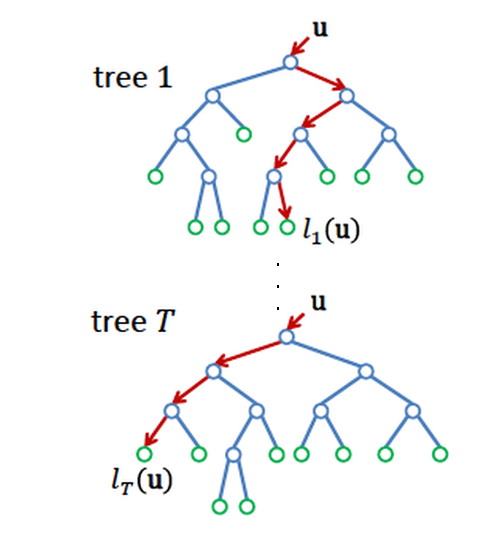
\includegraphics[width=\textwidth]{assets/forest.png}
\caption{Randomized Decision Forests}
\label{fig:decision_forests}
\end{subfigure}
\begin{subfigure}[b]{0.35\textwidth}
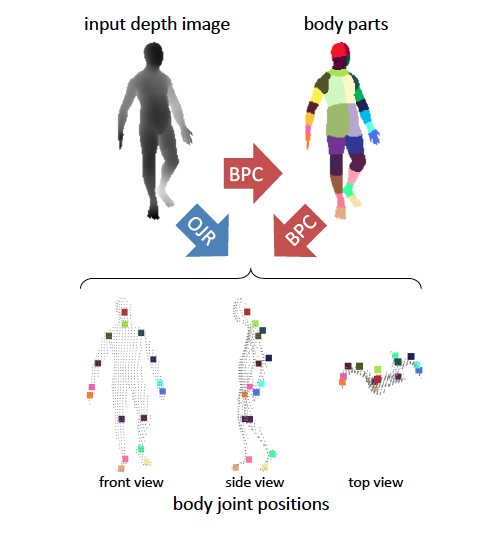
\includegraphics[width=\textwidth]{assets/kinect_approaches.png}
\caption{Human Pose estimation}
\label{fig:kinect_pose}
\end{subfigure}
\caption[Human pose estimation using single depth images]{Pose estimation using single depth images. {Adopted from \cite{shotton2013efficient}}}
\end{figure} 
\subparagraph{Body Part Classification} % (fold)
\label{subp:bpc} 
The first approach employs an intermediate body parts representation, designed so that an accurate per-pixel classification of the parts will localize the joints of the body. It transforms the pose estimation problem into one that can be readily solved by classification algorithms. For the classification, \emph{31} body parts are defined: LU/RU/LW/RW head, neck, L/R shoulder, LU/RU/LW/RW arm, L/R elbow, L/R wrist, L/R hand, LU/RU/LW/RW torso, LU/RU/LW/RW leg, L/R knee, L/R ankle, and L/R foot (Left, Right, Upper, Lower). The classification forest used for Body Part Classification (BPC) uses a probability mass function(PMF) - $p_l(c)$ over body parts $c$ as the prediction model. The classification forest helps achieve the per-pixel classification by storing a distribution $p_l(c)$ over the discrete body parts $c$ at each leaf $l$. For a given input pixel $u$, the tree is descended to reach leaf $l = l(u)$ and the distribution $p_l(c)$ is retrieved. The distributions are averaged together for all trees in the forest to give the final classification as
\begin{equation}
p(c\vert \textbf{u}) = \frac{1}{T}\sum_{l\in L(\textbf{u})} p_l(c)
\label{eqn:bpc_dist}
\end{equation}
Where $p_l(c)$ is PMF at the leaf node corresponding to body part $c$, $u$ is input pixel and $T$ is number of decision trees. The image space predictions are next re-projected into world space. The re-projection function is denoted as $x(u) = (x(u); y(u); z(u))^\text{T}$. Conveniently, the known $z(u)$ from the calibrated depth camera allows to compute $x(u)$ and $y(u)$ trivially. The body parts inherently lie on the surface of the body, thus a learned per-joint vector ${\zeta_j} = (0,0,\zeta_j)^\text{T}$ is used to push back the re-projected pixel surface positions into the world to better align with the interior joint position: $x_j(u) = x(u) + {\zeta_j}$. 
\subparagraph{Offset Joint Regression} % (fold)
\label{subp:ojr}  
The second approach presented in \cite{shotton2013efficient} directly regresses the positions of body joints. The ground truth labels required for this approach are simply the ground truth 3D joint positions which are recorded during the mesh skinning process. In this approach \emph{16} body joints are defined: head, neck, L/R shoulder, L/R elbow, L/R wrist, L/R hand, L/R knee, L/R ankle, and L/R foot. The regression forest used for Offset Joint Regression (OJR) uses a set of weighted relative votes $V_{lj}$ for each joint $j$. At each leaf node $l$ a distribution over the relative 3D offset from the re-projected pixel coordinate $x(u)$ to each body joint $j$ of interest is stored. Each pixel can thus potentially cast votes to all joints in the body, and unlike BPC, these votes may differ in all world space coordinates and thus directly predict interior rather than surface positions. The distribution at the leaf node is represented using a \emph{small} set of 3D \emph{relative vote} vectors $\Delta_{ljk} \in \Re^3$. The subscript $l$ denotes the leaf node, $j$ denotes a body joint and $k \in \lbrace 1,...,K \rbrace$ denotes the maximum number of relative votes allowed. A confidence weight $w_{ljk}$ is associated with each vote and it is critical for the accuracy. The set of relative votes for joint $j$ at the node $l$ is denoted as $V_{lj}={{\lbrace (\Delta_{ljk},w_{ljk}) \rbrace}^K}_{k=1}$. In order to improve the speed, $N_{sub}$ samples could be obtained from ${X_j}^{OJR}$ by either random sampling or picking top $N_{sub}$ samples from it. 
\subsubsection{Estimation using both Depth and RGB image}
Unlike the approaches used in the Kinect SDK, the approach presented in \cite{buys2014adaptable} uses both the depth and color (RGB-D) data for human body detection and pose estimation using a customizable human kinematic model. Other merits include the requirement of less training data and open source nature of this approach. 
\begin{figure}[H]
\centering
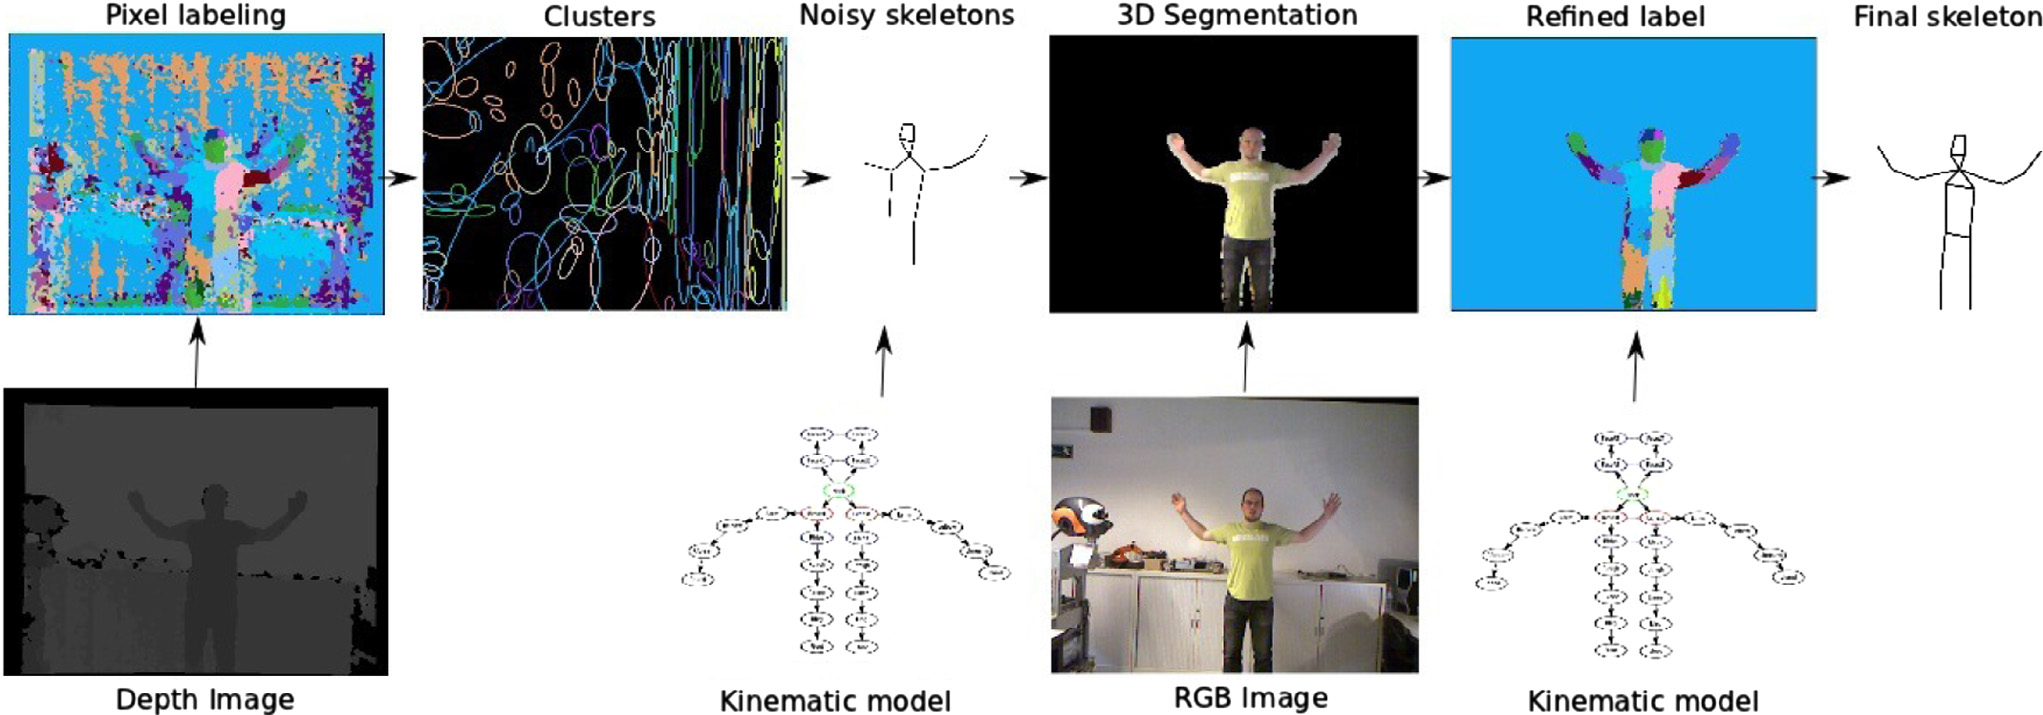
\includegraphics[width=\textwidth]{assets/adaptable_system_rgbd.png}
\caption[Adaptable system for human body detection and pose estimation]{Adaptable system for human body detection \& pose estimation. {Adapted from \cite{buys2014adaptable}}}
\label{fig:adaptable_rgbd}
\end{figure}
The goal of this approach is to output the 3D locations of the human body parts that are predefined in a kinematic model using the data received from an RGB-D sensor. The higher level process flow diagram of the system is shown in Figure~\ref{fig:adaptable_rgbd}. To start with, for a single depth map frame, per-pixel labeling is done using the similar approach described in\cite{shotton2013real}. However the principal difference is that no \emph{background subtraction} or fixed-pose initialization step before pixel labeling. A body part proposal step is performed on the initial noisy result, which results in a more robot part estimates. Using the statistical inference of the part estimates, a search for feasible kinematic trees is conducted during the kinematic tree search step. This result in the person detections and noisy skeletonization. In order to improve the obtained estimate, a second iteration of per-pixel body part labeling, body part proposal and kinematic tree search is performed. An appearance model is estimated online for segmentation refinement step. The noisy initial estimate obtained during the first iteration is used as a seed for color and depth-based segmentation that retrieves missing body parts and better localizes existing parts. This process can be used for multiple people among clutter and occlusion. This algorithm has been implemented as part of the PCL\cite{rusu20113d} library under the name \emph{People's library}.

\subsection{Gesture Recognition}
	Understanding of human motion is not complete if the gesture of the human could not be understood. The next step after the human pose is tracked is to recognise the gesture. Hidden Markov models (HMM) which had been widely used for speech recognition\cite{rabiner1989tutorial} also inspired to be used for the gesture recognition applications. The HMM model is generated for each motion primitives and Viterbi algorithm is used to find the optimum sequence of the states given a set of observations. During the recognition step a likelihood function is used on the segmented motion pattern against each HMM and the motion primitive corresponding to HMM with large likelihood is selected as shown in Figure~\ref{fig:hmm}. Auto segmentation of arm motion and recognition of motion patterns using angular velocity data obtained by IMU sensors and the Wii remote using HMM has been demostrated in \cite{aoki2013segmentation}. 
\begin{figure}[H]
\centering
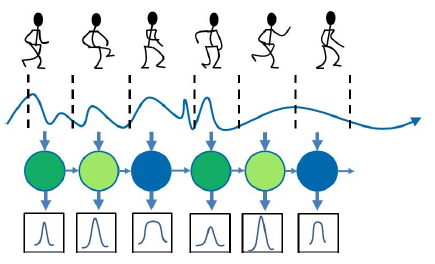
\includegraphics[width=0.3\textwidth]{assets/HMM.png}
\caption[HMM motion modeling]{HMM motion modeling. {Adapted from \cite{aoki2013segmentation}}}
\label{fig:hmm}
\end{figure}
In the publication by Microsoft research \cite{han2013enhanced}, a background study on various algortihms used for human activity analysis is presented. Recently \cite{KinectSDK2014} data-driven machine learning approaches like neural networks, Support vector machines, clustering, decision trees and bayesian networks are being exploited to this purpose. In \cite{KinectSDK2014}, an Adaptive Boosting algorithm\cite{freund1997decision} which is one of the top 10 data mining algorithms, is used to efficiently detect the gestures. The system involves a training phase in which the desired gestures are captured and tagged. These tagged gestures will be used by a gesture detector trainer which will generate a set of training examples $S=\lbrace \lbrace x_n,y_n \rbrace,\ n=1,\cdots,N \vert x_n\in X,y_n\in Y, X=\text{skeleton},Y=\lbrace -1,+1 \rbrace\rbrace$, associated data and set of weak classifiers $h_t$ and it learns the confidence $\alpha_t$ for $h_t$. The training results are stored in files and will be used by the gesture detector to perform per-frame classification of the data using $(h_t,\alpha_t)$. This approach has been proved to be robust with accuracy as high as 94.9\%. 

\section{Localization of Humanoid Robot} % Main chapter title
The localization of humanoid robots is a challenging issue, due to rough odometry estimation, noisy onboard sensing, and the swaying motion caused by walking \cite{cervera2012localization}. As a prelimnary assumption, the link of the robot are considered \emph{rigid bodies} in which distance between any two given points on it remains constant in time regardless of external forces exerted on it. Rigid body transformation forms the basic components in the pose estimation framework. In the $3D$ operational space represented by the vector space $\Re^3$, a rigid body is represented by \emph{6 degrees of freedom (DOF)}, 3 for the position along each of the coordinate axes (cartesian coordinates) $P = [p_x,p_y,p_z]^{\text{T}}$ and 3 for the orientation $R$. There are different representation for the orientation of the rigid body. They are rotation matrices, euler angles, RPY (roll,pitch,yaw) angles, quaternions. A detailed introduction about rigid body mechanics and various representation of pose of a rigid body can be found in the book by Khalil\cite{khalil2004modeling}.For most of the humanoid robots the reference frame will be fixed to the torso as is the case for the Nao. So the basic idea is to track the torso of the Nao or any other position with the known transformation from the torso. In this section different techniques that could be effectively used for localization and tracking of the humanoid robot are presented.

\subsection{Artificial Marker based approaches}
The advancements in the field of augmented reality led to the development of efficient tracking of object poses by employing fiducial markers. Tracking rectangular fiducial markers can be interesting if we could embed those markers on the humanoid robot. This is one of the simplest and cheapest solution in terms of the computational power as it uses simple image processing algorithms. ARToolKit\cite{kato1999marker} implements video tracking libraries which can calculate the real camera position and orientation relative to physical markers in real time. Before camera-based 6DOF tracking can be performed, the camera must be calibrated once as a pre-processing step. The perspective projection and the camera distortion parameters obtained during this step will be used later during the tracking initialization phase. During the tracking, as a first step ARToolKit performs a very simple edge detection by thresholding the complete image with a constant value, followed by a search for quadrangles. Resulting areas being either too large or too small are immediately rejected. Next the interior areas of the remaining quadrangles are normalized using a perspective transformation. The resulting sub-images are then checked against the set of known patterns. When a pattern is detected, ARToolKit uses the marker’s edges for a first, coarse pose detection. In the next step the rotation part of the estimated pose is refined iteratively using matrix fitting. The resulting pose matrix defines a transformation from the camera plane to a local coordinate system in the centre of the marker. ARToolKit can combine several co-planar markers into a multi-marker set. From an application point of view this multi-marker set is treated as a single marker and can be tracked as long as one or more markers of this set are visible. Multi-marker tracking increases the computational load but results in considerably more accurate and robust tracking. ARToolKit also gives the possibility for user-defined markers and the libraries could be trained to track those markers in real time.
\begin{figure}[H]
\centering
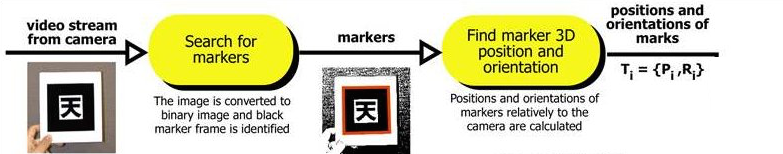
\includegraphics[width=1\textwidth]{assets/artoolkit.eps}
\caption[Marker tracking using ARToolKit]{Marker tracking using ARToolKit. {Adapted from \cite{kato1999marker}}}
\label{fig:artoolkit}
\end{figure}
\subsection{Point Cloud based approaches}
\label{ssec:pcl}
The Point Cloud Library (PCL)\cite{rusu20113d} which is one of the most widely used 3D perception software library, has collection of state-of-the-art algorithms and tools to process 3-D data. The library is open source and licensed under Berkeley Software Distribution (BSD) terms and, therefore, free to use for everyone. 
\subsubsection{PCL Pose estimation Pipeline}
	Point cloud library provides an excellent infrastructure for the object recognition and 6DOF pose estimation pipeline by offering a wide variety of robust local and global features. A list of features available is presented in \cite{aldoma2012point}. Object recognition based on global/local features almost share the same flow of operations. A glimpse of the pipeline is shown in Figure~\ref{fig:pcl_pipeline}.
\begin{figure}[H]
\centering
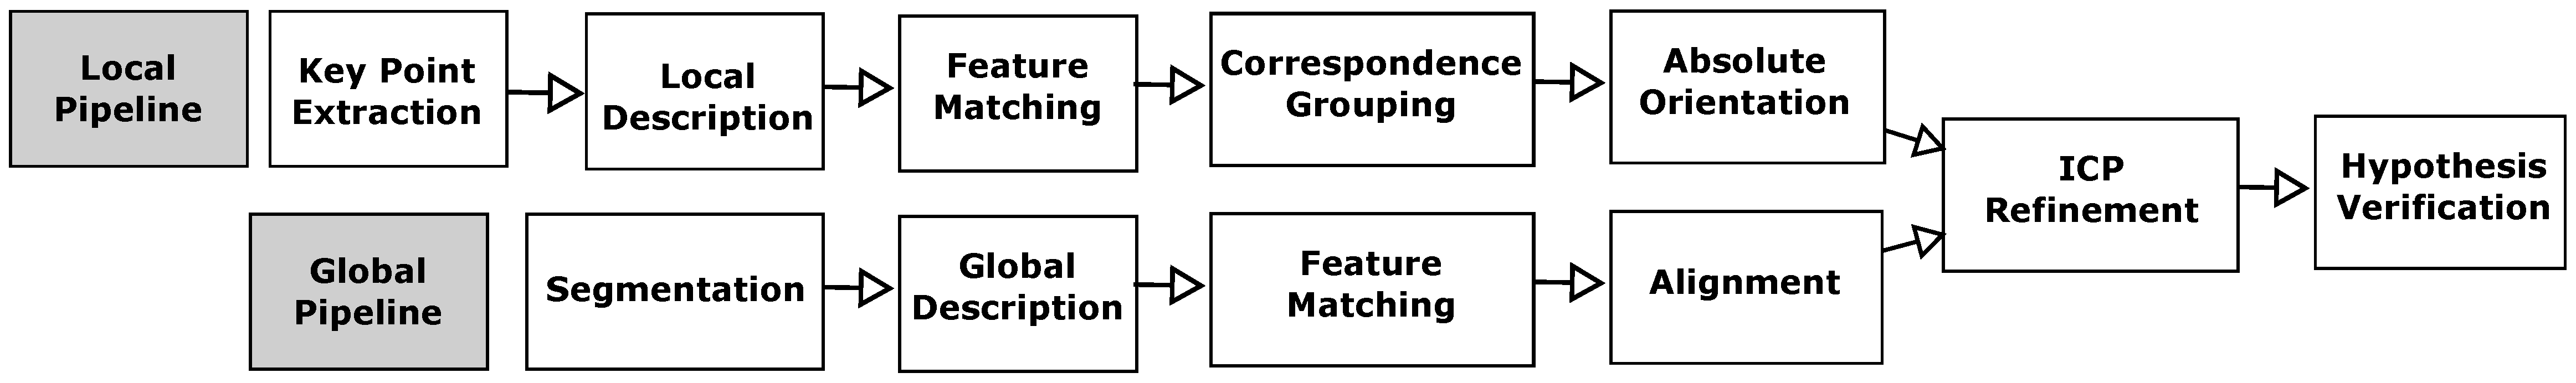
\includegraphics[width=1\textwidth]{assets/pcl_pipeline.eps}
\caption[PCL local and global 3D Pipelines]{PCL local and global 3D Pipelines. {Adapted from \cite{aldoma2012point}}}
\label{fig:pcl_pipeline}
\end{figure}
Before the PCL system being able to detect the pose of the object, the system has to be trained with the point clouds of the meshes generated by a virtual depth camera. The 3D features of the model are computed and stored to be used during the recognition phase. The first step in the recognition based on \emph{local descriptors} is \emph{key-point extraction} which detect repeatable and distinct key points from the scene data. After this step, they are associated to a \emph{local description} defined over a local support for determining the subset of neighbouring points around the key point. Once descriptor are computed for the current scene and each model in the library, \emph{matching} will be performed to yield point-to-point correspondences. This is followed by an additional stage called \emph{correspondence grouping} during which correspondence which are not geometrically consistent are discarded. However this step does not guarantee that all remaining correspondences are consistent with unique 6-DOF pose. To this purpose Random Sampling Consensus (RANSAC) is used to remove the outliers. Following this, a least square optimization is performed to obtain the rotation and the translation from exact point correspondences. For recognition based on global descriptors, the first step involves a \emph{segmentation} of the scene to extract the objects in it based on the extraction of a dominant scene plane and euclidean clustering step. During the \emph{description and matching} steps, the shape and geometry of each objects in the scene are described using appropriate global descriptor and represented by one or more histograms. The histogram \emph{matching} is done to those obtained during training stage to retrieve $N$-nearest neighbors using \emph{FLANN (Fast Library for Approximate nearest neighbors)}. An aliging step following this will give a 5-DoF pose since the global descriptors are invariant to roll axis rotation. This rotation could be achieved using \emph{camera roll histogram}.Both the global and local pipelines can undergo an optional \emph{post processing} step by applying Iterated Closest Point (ICP) in order to refine estimated 6-DoF pose. The following step referred to as \emph{hypotheses verification} which aims at reducing false positives(FPs).
\subsubsection{PCL Tracking pipeline}
Apart from the object recognition and pose estimation pipeline, PCL provides a comprehensive algorithmic base for the tracking of 3D objects using Monte Carlo sampling techniques \cite{RUeda2012} and for calculating the likelihood using combined weighted metrics for hyperdimensional spaces including cartesian data, colors, and surface normals. PCL also has non-probabilistic tracking algorithms like Pyramidal Kanade Lucas Tomasi (KLT) Tracker in its tracking module. The KLT tracker operates on organized 3D keypoints with color/intensity information. A list of probabilistic tracking algorithms implemented in PCL is presented in Section~\ref{sssec:prob_solutions} for the purpose of being coherent.
\subsection{Probabilistic Approaches}
\label{ssec:prob_approaches}
Probabilistic localization algorithms are variants of the Bayes filter \cite{thrun2005probabilistic}. The pose of the robot is represented in a probabilistic manner called the \emph{belief}: ($bel(x_t)$) which is a posterior distribution over the state space. The basic principle behind Bayes filter is that the belief $bel(x_t)$ at time $t$ is calculated from the belief $bel(x_{t-1})$ at time $t-1$ along with the most recent control $u_t$ and the most recent measurement $z_t$. It involves two basic steps: \emph{Control update step} during which the $\overline{bel(x_t)}$ is computed based on the prior assigned to $x_{t-1}$ and the probability that control $u_t$ induces a transition from $x_{t-1}$ to $x_t$, \emph{Measurement update step} during which the hypothetical posterior $\overline{bel(x_t)}$ is multiplied with the probability of seeing an observation $z_t$ given this $x_t$. The recursive computation of belief state can thus be given by
\begin{align*}
\text{Control update step:}\quad \overline{bel(x_t)} &= \int p(x_t\vert u_t,x_{t-1})\cdot bel(x_{t-1}) dx \\
\text{Measurement update step:}\quad {bel(x_t)} &= \eta\cdot p(z_t\vert x_{t})\cdot \overline{bel(x_t)}
\end{align*}
where $\eta$ is the normalization factor. The straightforward application of Bayes filters to the localization problem is called Markov localization. Markov localization makes use of the \emph{Markov assumption} (The Markov assumption postulates that past and future data are independent if one knows the current state {$x_t$). Extended Kalman Filter(EKF) based localization is one of the initial developments to be used in non-linear state models. However they suffered problems of uni-modal distribution(gaussian) assumption and failing to solve global localization problem. In the following section, a class of non-parametric localization approach is presented. 
\subsubsection{Particle Filter}
\label{ssec:particlefilter}
	The particle filter\cite{thrun2005probabilistic} is an alternative non parametric implementation of Bayes filter. The key idea of the particle filter is to represent the posterior $bel(x_t)$ by a set of samples drawn from the distribution. Such a representation is approximate, but it is nonparametric, and therefore can represent a much broader space of distributions than, for example, Gaussians. The important components of a particle filter are\\
\begin{tabular}{r l}
\centering
  (Control input,Measurement) & $(u_t,z_t)$ \\ 
  Sample of Posterior distribution (particles) & $X_t := {x_t}^{[1]},{x_t}^{[2]},\cdots,{x_t}^{[M]}$ \\
  (Posterior PDF,Likelihood function) & $(p(X_t\vert z_{1:t}),p(z_t \vert {x_t}^{[m]})$ \\
  Importance Factor of $m^{th}$ particle & ${w_t}^{[m]}$ \\
\end{tabular}
	
	Each particle ${x_t}^{[m]}$ (with $1 \leq m \leq M$) is the concrete instantiation of the state at time $t$, that a hypothesis as to what the true world state may be at $t$. Here $M$ denotes the number of particles in the set $X_t$. The basic intuition behind the particle filter is to approximate the belief $bel(x_t)$ by the set of particles $X_t$ and as a consequence denser a subregion of the state space is populated by samples, the more likely the true state falls in the region.The current state is given by the weighted particle mean 
\begin{equation}
E(X_t) = \sum_{m=1}^{M} {w_t}^{[m]}\cdot {x_t}^{[m]}
\end{equation}
The basic algorithm of particle filter is shown in \ref{alg:particlefilter}.\\ 
\begin{algorithm}
\KwData{$X_{t-1}$, $u_t$, $z_t$}
\KwResult{$X_t$}
Init: {$\tilde{X_t}$ = $X_t$ = $\emptyset$ } \;
 \For{$m$ = $1$ to $M$} { 
   sample ${x_t}^{[m]} \approx p(x_t \vert u_t,{x_{t-1}}^{[m]}) $ //Hypothetical state computation \;
   ${w_t}^{[m]} = p(z_t \vert {x_t}^{[m]} )$ //Importance factor computation\;
   $\tilde{X_t} = \tilde{X_t} + ({x_t}^{[m]},{w_t}^{[m]})$ \;
 }
 \For{$m$ = $1$ to $M$} { 
   draw $i$ with probability $\varpropto$ ${w_t}^{[i]}$ //Importance re-sampling\;
   add ${x_t}^{[i]}$ to $X_t$ \;
 }
 return $X_t$
 \caption{Basic algorithm of Particle Filter}
 \label{alg:particlefilter}
\end{algorithm}
\subsubsection{Monte Carlo Localization}
\label{ssec:montecarlo}
	Monte-carlo localization (MCL)\cite{fox1999monte} is a version of Markov localization, a family of probabilistic approaches that has been successfully applied to localization problems and it has become one of the most popular localization algorithms in robotics. MCL uses fast sampling techniques to represent the belief and it introduces probabilistic motion and perceptual models into the particle filter framework. Hence it uses the same formalism described in \ref{ssec:particlefilter}.\\  	
\begin{algorithm}
\KwData{$X_{t-1}$, $u_t$, $z_t$}
\KwResult{$X_t$}
Init: {$\tilde{X_t}$ = $X_t$ = $\emptyset$ } \;
 \For{$m$ = $1$ to $M$} { 
   ${x_t}^{[m]} = \text{sample\_motion\_model}(u_t,{x_{t-1}}^{[m]})$ //Hypothetical state computation\;
   ${w_t}^{[m]} = \text{measurement\_model}(z_t,{x_t}^{[m]},m)$ //Importance factor computation \; 
   $\tilde{X_t} = \tilde{X_t} + ({x_t}^{[m]},{w_t}^{[m]})$ \;
 }
 \For{$m$ = $1$ to $M$} { 
   draw $i$ with probability $\varpropto$ ${w_t}^{[i]}$ //Importance re-sampling\;
   add ${x_t}^{[i]}$ to $X_t$ \;
 }
 return $X_t$
 \caption{Monte Carlo Localization}
 \label{alg:montecarlo}
\end{algorithm}

	The efficiency of particle filters lies in the way they place computational resources. By sampling in proportion to likelihood, particle filters focus the computational resources on regions with high likelihood, where good approximations are most important. The time complexity of one update of the particle filter algorithm is linear in the number of samples needed for the estimation. The Kullback-Leibler Distance(KLD) adaptive sampling technique proposed in \cite{fox2003adapting} presents an approach to adapt the number of samples over time. The key idea is at each iteration of the particle filter, the number of samples are determined such that, with probability $1-\delta$, the error between the true posterior and the sample-based approximation (maximum likelihood estimate- MLE) is less than $\epsilon$. The distance between the MLE and the true distribution is measured by a non-negative Kullback-Leibler distance which for two distributions $p$ and $q$ is given by
\begin{equation}
K(p,q) = \sum_{x} p(x)log{\frac{p(x)}{q(x)}}
\end{equation}

\subsection{Existing Solutions}
\label{sssec:prob_solutions}
	\par The Point cloud library \cite{RUeda2012} introduced in Section~\ref{ssec:pcl} implements ready to use probabilistic tracking algorithms like: the most basic particle filter tracker(\emph{ParticleFilterTracker}), particle filter using OpenMP support(\emph{ParticleFilterOMPTracker}), KLD-adaptive sampling particle filter( \emph{KLDAdaptiveParticleFilterTracker}) and KLD adaptive sampling with OpenMP support ( \emph{KLDAdaptiveParticleFilterOMPTracker}). This could be readily used to track an object of know geometry and this information has to be fed to the PCL through a point cloud mesh of the object.
	
	Studies on robot localization, obstacle mapping, and path planning in multilevel 3D environments by equipping Nao with a consumer-level depth camera has been reported in \cite{maier2012real}. This study provides real-time solution while maintaining a 3D environment representation and estimating the robot’s pose in 6D. The 3D environment model in form of an octree based representation containing the static parts of the environment is used. In this representation, the robot estimates its pose using MCL based on acquired depth data. Given the estimated 6D pose of the humanoid and a sequence of depth images, this approach continuously builds a local 3D representation of the current state of the environment containing also non-static obstacles. This learned octree-based representation is then used for real-time planning of collision-free paths. For robust localization while walking, it combines 3D range data from the depth camera located on top of the head, altitude data provided by an inertial measurement unit (IMU) in the chest and odometry data.
	
	While \cite{maier2012real} presented an approach wherein a depth camera is fixed to the humanoid robot, in \cite{cervera2012localization} localization and motion planning in smart home environment have been proposed. In this study an external depth camera is used for 6D pose estimation and tracking, which is very close to the scenario of this thesis. Once again MCL technique is used for the pose estimation of the torso of the humanoid robot and this information is used for the closed loop navigation control. For the localization, this study used  \emph{KLDAdaptiveParticleFilterOMPTracker} available in Point cloud library. For the purpose of navigation, this study determined the pose error on the plane of walking using the knowledge of estimated pose and the desired pose. The linear velocity of the robot is calculated from the pose error using a proportional gain. The angular velocity is determined adaptively depending on the distance to the target. The localization results of this study proved to be robust compared to the odometry data. However this study did not take into account of collision free navigation planning. 
	
	In \cite{choi2013rgb} a robust particle filter parallelized on a GPU that can track a known 3D object model over a sequence of RGB-D images is proposed. This method proposes to render the 3D object model to be used in the likelihood function so that the object could be tracked inspite of significant pose variations. Unlike PCL object tracking algorithm\cite{rusu20113d} which maintains only one reference point cloud, this approach uses multiple viewports rendered in GPU with different poses and each particle searches the closest rendering from the viewports and likelihood evaluation is performed by transforming the closest rendered result with the current particle state. Each particle is defined as 6D vector consisting of position and orientation of the object. For the likelihood evaluation, this work exploits the RGB-D data and utilizes the position, normal and color information of the points. Through a set of extensive experiments with both synthetic and real RGB-D sequences, this approach has been proved to be faster and also accurate than the PCL tracking.
	
\section{Behavioral Frameworks} % Main chapter title
The users of social robots do not have necessary backgrounds in programming and design of robot behaviors. This lead to the development of several visual programming languages which allow non-programmers to create robot applications. Most of the available visual programming softwares allows to choose among many prebuilt behavioral blocks and connecting them to one another to get the desired flow of action \cite{MSRS4},\cite{Choregraphe}. These programs are very intuitive and allow the users to realize complex sequence of movements and sequential behaviors. But programming dynamic behaviors still remains challenging. This is primarily due to fact that the users have to think about the data flow between various blocks by appropriate connections between them. When it comes to designing complex dynamic behaviors this task becomes very tedious and time consuming.  Programming complex dynamic behaviors for small commercial humanoid robots is a complicated task for the inexperienced roboticists \cite{berenz2014targets} for the reasons such as synchronizing the data flows, conditional selection of actions, ensuring robustness and task continuity etc., There are many solutions  proposed in the literature that address the dynamic control problem. For instance Gostai's Universal Robotic Body Interface(URBI) \cite{baillie2008urbi} and Task description language (TDL) \cite{simmons1998task} are programming languages developed specifically for robot programming. URBI provides a modern object-oriented scripting language that allows the organization of code into different processes that either run sequentially or in parallel, and it also provides tools for process execution monitoring. In TDL which was developed as a C++ extension, the code is organized into task trees, which encode the hierarchical decomposition of tasks as well as the synchronization of constraints between tasks. More recently, specialized operating systems have been proposed, such as ROS \cite{quigley2009ros}, which organize code into distributed asynchronous modules that exchange data using a data subscription protocol. Hierarchical organization of behaviors and modularity are also being investigated \cite{jaeger1998dual} \cite{Baldassarre:2013:CRM:2560111} \cite{hurdus2008behavioral}. These solutions manage the integration and communication between different types of hardware and software and support the implementation of reaction, as well as behavioral specification. However, these programs have been produced by robot developers and are targeted at this community, which means that they are not intended to be used by non-roboticists and a solid background in computer science/robotics is required for their use.
\begin{figure}[H]
\centering
\begin{subfigure}[b]{0.5\textwidth}
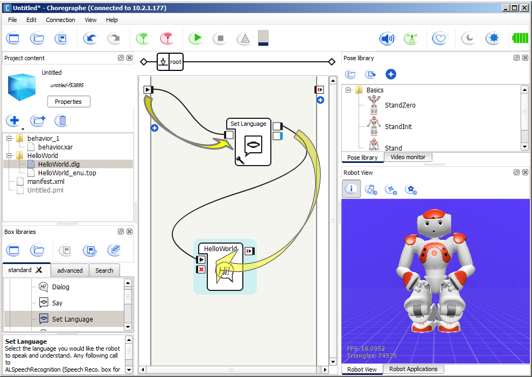
\includegraphics[width=\textwidth]{assets/helloworld_cho_dlg_05.png}
%http://doc.aldebaran.com/2-1/getting_started/helloworld_choregraphe_dialog.html
\caption{Choreographe Albebaran}
\label{fig:choreographe}
\end{subfigure}%
\begin{subfigure}[b]{0.5\textwidth}
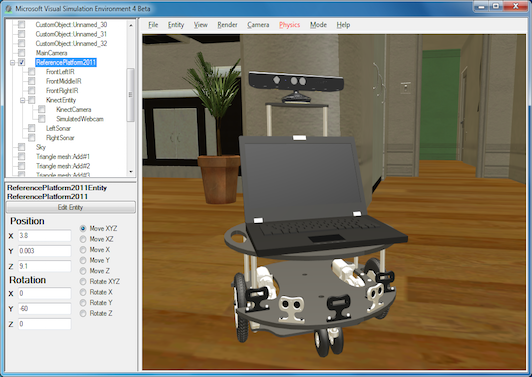
\includegraphics[width=\textwidth]{assets/MSRD4_VSE2.png}
%http://www.microsoftstore.com/store/msusa/en_US/pdp/Kinect-for-Windows-v2-Sensor/productID.298810500
\caption{MSRD Studio 4:Visual Simulation Environment}
\label{fig:msrd4_vse}
\end{subfigure}%
\caption[Visual Programming Tools]{Visual Programming Tools. {Adapted from manufacturer's site}}
\label{fig:visprog}
\end{figure}
A new non-domain-specific solution called \emph{Target Drives Means (TDM)} shown in Figure~\ref{fig:tdm_im} is proposed in \cite{berenz2014targets} taking into account the following requirements. TDM proposes a programming paradigm where temporal independent dynamic behaviors blocks run in parallel. The logic of the program is not expressed using communication links in a flowchart, but by the use of specialized dynamic components that regulate the activation status and the priorities of the behaviors. THe information exchange occurs via a specialized centralized memory called \emph{Internal Model(IM)} which takes care of asynchronous information flow (push/pull communication) between connected components, odometry, object permanence, and activation of behaviors through triggers. 
\begin{figure}[H]
\centering
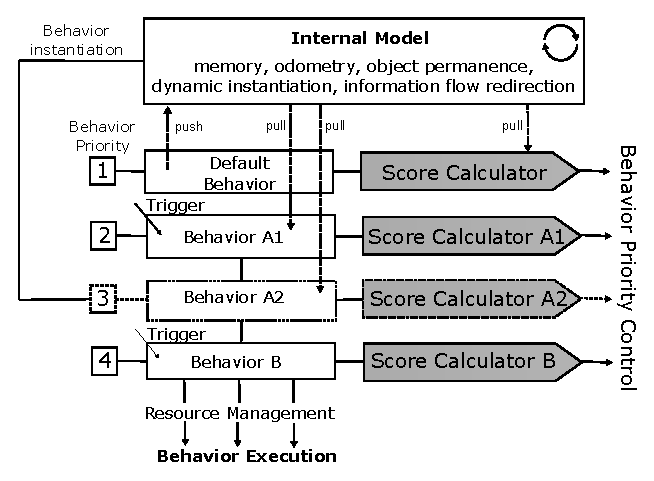
\includegraphics[width=0.5\textwidth]{assets/tdm_im.eps}
\label{fig:tdm_im}
\caption[Target-drives-means Framework]{TDM Framework. {Adapted from \cite{berenz2014targets}}}
\end{figure}
The comparison results of TDM and Aldebaran Choreographe presented in \cite{berenz2014targets} indicates that TDM is appropriate when it comes to designing complex dynamic behaviors. However there does not exist an intuitive interface for the behavior design yet and the framework is also not open and protected by intellectual property.

\section{HRI Design and Evaluation} % Main chapter title
Human-Robot Interaction (HRI) being a rapidly advancing area of research, there is a growing need for strong experimental designs and methods of evaluation. This will bring credibility and validity to scientific research that involves humans as subjects, as recognized in the psychology and social science fields. Some methods of evaluation have been adopted and/or modified from such fields as human-computer interaction, psychology, and social sciences; however, the manner in which a human interacts with a robot is similar but not identical to interactions between a human and a computer or a human interacting with another human. It often has a strong social or emotional component — a difference that poses potential challenges related to the design and evaluation of HRI. As robots are becoming more prevalent, accurate methods to assess how humans respond to robots, how they feel about their interactions with robots, and how they interpret the actions of robots are very important. 
%\subparagraph{Planning, Design and Data collection}
A successful human study in HRI requires careful planning and design. In \cite{bethel2010review}, a set of questions when planning and designing a human study in HRI is presented. Apart from providing a checklist for planning and design of HRI studies, a list of recommendations for the experimental design and study execution is also provided in \cite{bethel2010review}.
	
Data collection is one of the important steps in the evaluation process. In \cite{Rogers2011} which provides insights into designing interative systems, five key issues in the data gathering has been described. They are 
\begin{itemize}
\item \emph{Identifying participants} : Decide who to gather data from
\item \emph{Relationship with participants} : Establishing a clear and professional relationship
\item \emph{Setting goals} : Deciding how to analyze data once collected, Informed consent when appropriate
\item \emph{Triangulation} : Looking at data from more than one perspective
\item \emph{Pilot studies} : Small trial of main study. 
\end{itemize}
An extensive review of HRI evaluation methods presented in \cite{bethel2010review} summarises five primary methods such as \emph{Self assessments}, \emph{Interviews}, \emph{Behavioral Measures}, \emph{Psychophysiology measures}, \emph{Task performance metrics}. Each of these methods has advantages and disadvantages. However the study claims that it is possible to overcome these disadvantages by using three or more appropriate methods of evaluation. An effort to identify a set of common metrics to be used in task-oriented HRI can be found in \cite{Steinfeld2006}. This study proposes a set of metric to evaluate the human-robot team and human-robot interactions and those proposed metrics are shown in Table~\ref{table:hri_metrics}
\begin{table}[H]
\centering
\small
\caption{Common Metrics for task-based HRI}
\label{table:hri_metrics}
\begin{tabularx}{400pt}{c*3{X}}
\toprule
  \textbf{Common metrics} & \textbf{Sub-metrics} 
                          & \textbf{Description}
  \tabularnewline \midrule
  
  \multirow{4}{*}{System Performance} & Quantitative performance & Quantitative measures assess the
effectiveness and efficiency of the team at performing a task \\
                                      & Subjective ratings & Subjective ratings assess the quality
of the effort \\
                                      & Utilization of mixed-initiative & Ability of the human-robot team to appropriately regulate who has control initiative 
                                          \tabularnewline\midrule
                                          
  \multirow{4}{*}{Operator Performance} & Situation Awareness (SA) & The degree to which the robot is situation aware. It is critical for effective decision-making \\
                                      & Workload & Multidimensional workload assessment techniques are useful for relating human perceptions of cognitive load to operator SA \\
                                      & Accuracy of mental models & Impact of Design affordances, operator expectations and stimulus-response compatibility.
                                          \tabularnewline\midrule
  
  \multirow{4}{*}{Robot Performance} & Self Awareness & The degree to which a robot can accurately
assess itself \\
                                      & Human Awareness & The degree to which the robot is aware of humans \\
                                      & Autonomy & The ability of robots to function independently without human intervention.
                                          \tabularnewline                                
                                         
  										\bottomrule
\end{tabularx}
\end{table}
Bartneck et al.,\cite{bartneck2009measurement} emphasize the need for standardized measurement tools for human robot interaction. The main contribution of this work is that it presents measurements tools of five key concepts in HRI: anthropomorphism, animacy, likeability, perceived intelligence, and perceived safety. The outcome of the work is basically five consistent questionnaires using semantic differential scales. Moreover the study also reported reliability and validity indicators based on several empirical studies that used these questionnaires. Specifically, this study uses \emph{Cronbach's alpha} to estimate the reliability of the questionnaires. The results presented in the study showed that the developed questionnaires to measure the aspects have sufficient internal consistency reliability. All the evaluation techniques rely on the statistical tools for validating the results and generalizing the phenomena. A summary of statistical tools for the data analysis in HRI can be found in Appendix~\ref{AppendixA}.